\documentclass{article}
\usepackage{amsmath}
\usepackage{listings}
\usepackage{moreverb}
\usepackage[margin=1in]{geometry}
\usepackage{graphicx}
\usepackage{dsfont}
\title{STA 360: Assignment 2}
\author{Michael Lin}

\begin{document}
\maketitle

\begin{enumerate}
\setcounter{enumi}{3}
\item The 0-1 loss function is given by
$$ l(S,a) = \mathds{1}(S\neq a) $$
Therefore, the posterior expected loss is
$$ \mathds{E}(l(S,a)|x_{1:n}) = 1 \cdot \mathds{P}(S\neq a|x_{1:n}) + 0 \cdot \mathds{P}(S=a|x_{1:n}) $$
To minimize the posterior expected loss, we would need to find $a$ that would minimize $\mathds{P}(S\neq a|x_{1:n})$. Since the events $S\neq a$ and $S=a$ are mutually exclusive, minimizing the probability of the former event is equivalent to maximizing the probability of the latter. In particular, we would need the action $a$ that maximizes $\mathds{P}(S=a|x_{1:n})$, i.e.
$$ \delta(x) = \mathrm{argmax}_{a} \mathds{P}(S=a|x_{1:n}) $$

\item Since $x_1,...,x_n$ are Bernoulli random variables, the intuitive prediction of $x_{n+1}$ would be the mode of $x_1,...,x_n$, i.e., the value (either 1 or 0) that occurs more often.  Based on the previous problem, the Bayes procedure for making this prediction would be choosing the $a$ that would maximize $\mathds{P}(x_{n+1}=a|x_{1:n})$. Let $a_n=a+\sum x_i$ and $b_n=b+n-\sum x_i$. Thus, given the posterior distribution
$$p(\theta|x_{1:n})=\mathrm{Beta}(\theta|a_n, b_n)$$
the posterior predictive, from section 3.2 of notes, would be 
$$p(x_{n+1}|x_{1:n}) = \left\{
  \begin{array}{lr}
    \frac{a_n}{a_n+b_n} & \text{if } x_{n+1} = 1\\
    \frac{b_n}{a_n+b_n} & \text{if } x_{n+1} = 0
  \end{array}
\right.
$$
Therefore, the Bayes procedure is
$$\delta(x) = \mathrm{argmin}_a \rho(a,x) =\left\{
  \begin{array}{lr}
    1 & \text{if } \frac{a_n}{a_n+b_n}\geq \frac{b_n}{a_n+b_n}\\
    0 & \text{otherwise}
  \end{array}
\right.
$$

\item The hyperparameters would be $a,b$ such that
$$ \frac{a+\sum x_i}{a+b+n}\geq \frac{b+n-\sum x_i}{a+b+n} $$
But notice this is true for $a=b=0$. Thus this would be one such setting of the hyperparameters that agrees with the above Bayes procedure. The values $a$ and $b$ determine the posterior predictive and shift the intuitive choice. A larger $a$ shifts the prediction towards 1; a larger $b$ shifts the prediction towards 0.

\setcounter{enumi}{7}
\item The following Riemann sum with equal partition $\{x_0=0, x_1, x_2..., x_N=1\}$ was used to approximate an integral:
$$ \int\limits_{0}^{1} f(x)dx \approx \frac{1}{N} \sum\limits_{i=1}^{N} f(x_{i-1}) $$

Below is the plot of the posterior expected loss.
\begin{center}
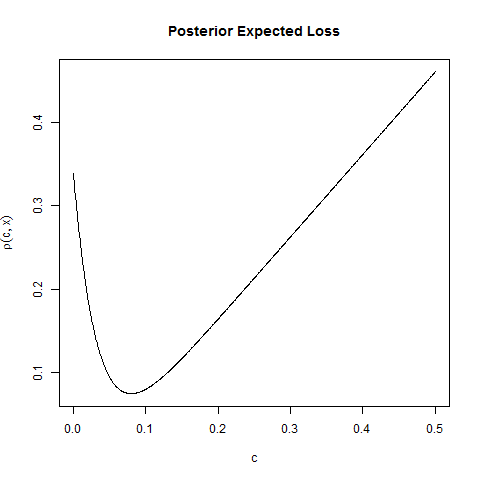
\includegraphics[scale=0.4]{pel.png}
\end{center}
\end{enumerate}

\pagebreak

See below for R code used to plot posterior expected loss.

\listinginput[1]{1}{assign2code.r}


\end{document}